\section{Appendix: CBN is a causal theory}\label{app:cbn_ct}

\begin{theorem}\label{th:cbn_MK}
Given a measurable set $(E,\mathcal{E})$ and a graph $\mathcal{G}$ over a set of random variables $\{\RV{X}^i\}_{i\in[N]}$ where $\RV{X}^i:E\to X^i$, a decision set $(D,\mathcal{D})$ and random variables $\{\RV{D}^i\}_{i\in[N]}$ with $\RV{D}^i:(D,\mathcal{D})\to (X^i\cup\{*\},\sigma(\mathcal{X}^i\cup\{*\})$. Given $\mu\in \mathscr{G}_{\mathcal{G}}$, let $\mu^y$ be the $\mathcal{G},\mu,y$-interventional distribution (Definition \ref{def:CBN}). 

Then the map $\kappa^{\mu,\mathcal{G}}:D\to \Delta(\mathcal{E})$ given by $y\mapsto \mu^y$ is a Markov kernel with respect to $(D,\mathcal{D})$ and $(E,\mathcal{E})$.
\end{theorem}

\begin{proof}
The DAG $\mathcal{G}$ induces a partial ordering on the RV's $\RV{X}^i$ by $\RV{X}^i < \RV{X}^j$ if 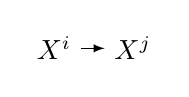
\begin{tikzpicture}[baseline=-1.5mm,-latex]
\node (C) {$\RV{X}^i$};
\node [right of = C] (A) {$\RV{X}^j$};
\draw (C) -- (A);
\end{tikzpicture} is in $\mathcal{G}$. Without loss of generality, suppose the total ordering $X^0,...,X^N$ is consistent with the partial ordering induced by $\mathcal{G}$.

Let $\kappa^i: \mathcal{E}\to \Delta(\mathcal{X}^i)$ be defined by $\kappa^i(x;A) := \mu_{\RV{X}^<i} F_{\RV{X}^i}$. Note that by the compatibility of $\mu$, for all $x\in \mathcal{E}$, $A\in \mathcal{X}^i$ we also have
\begin{align}
    \kappa^i(x;A) = \mu_{\PA{\mathcal{G}}{\RV{X}^i}} F_{\RV{X}^i} (x;A) \label{eq: compatibilty}
\end{align}

Consider $\kappa^{i,*}:D\times E \to \Delta(\mathcal{X}^i)$ given by \begin{align}
    \kappa^{i,*}(y,pa^i;A) := \begin{cases}\kappa^i(pa^i;A) &\RV{D}^i(y) = * \\
    \delta_{\RV{D}^i(y)}(A) & \RV{D}^i(y) \neq *\end{cases}\label{eq:passive}
\end{align}

Clearly for every $(d,pa^i) \in D\times E$ the map $A\mapsto \kappa^{i,*}(d,pa^i;A)$ is a probability distribution on $\mathcal{X}^i$. Fix $B\in\mathcal{X}_i$ and let $\kappa^{i,*}_B=\kappa'_i(\cdot;B)$.

Then for any $A\in \mathcal{B}([0,1])$
\begin{align}
    [\kappa^{i,*}_B]^{-1}(A) &= [\RV{D}^i]^{-1}(\{*\})\times[\kappa^B_i]^{-1}(A) &\text{if }0,1\not\in A\\
    &= [\RV{D}^i]^{-1}(\{*\})\times[\kappa^B_i]^{-1}(A)\cup [\RV{D}^i]^{-1}(B)\times X^{\PA{\mathcal{G}}{i}} &\text{if }1\in A\land 0\not\in A\\
    &= [\RV{D}^i]^{-1}(\{*\})\times[\kappa^B_i]^{-1}(A)\cup [\RV{D}^i]^{-1}(B^C)\times X^{\PA{\mathcal{G}}{i}} &\text{if }0\in A\land 1\not\in A\\
    &= [\RV{D}^i]^{-1}(\{*\})\times[\kappa^B_i]^{-1}(A)\cup [\RV{D}^i]^{-1}(X^i)\times X^{\PA{\mathcal{G}}{i}} &\text{if }0\in A\land 1\in A
\end{align}
Note that $\sigma(\PA{\mathcal{G}}{\RV{X}^i}\subset\mathcal{E}$ and $[\kappa^B_i]^{-1}(A)\in \sigma(\PA{\mathcal{G}}{\RV{X}^i}$. Further note that $\{*\}$, $B$ and $B^C$ are in $\sigma(\mathcal{X}^i\cup\{*\})$. Therefore, in every case the result is  an element of $\mathcal{E}\otimes\mathcal{D}$ and $\kappa^{i,*}$ is a Markov kernel.

Then $\iota^{\mathcal{G}}:D\to \Delta(\mathcal{X})$ defined below is a Markov kernel.
\begin{align}
    \iota^{\mathcal{G}}:(y;A)\mapsto \int_{A^0} \kappa^{0,*}(y;dx^0) ... \int_{A^{N-1}} \kappa^{N-1,*}(y,x^{n-2};dx^{n-1}) \kappa^{N,*}(y,x^{n-1};A^N) \label{eq:bigproduct}
\end{align}

for $y\in D$, $A\in E$ and $A^i= [\RV{X}^i]^{-1}(A)$.

From Equations \ref{eq: compatibilty}, \ref{eq:passive} and \ref{eq:bigproduct} we can verify that, given some $i\in N$, if $\RV{D}^i(y)=\{*\}$ then $[\delta_y \iota^{\mathcal{G}}]_{\PA{\mathcal{G}}{\RV{X}^i}} = \kappa_i = \mu_{\PA{\mathcal{G}}{\RV{X}^i}} F_{\RV{X}^i}$ and if $\RV{D}^i(y)\neq\{*\}$ then $\delta_y \iota^{\mathcal{G}} = \delta_{\RV{D^i}(y)} F_{\RV{X}^i}$. From Equation \ref{eq:bigproduct} and the compatibility of $\mu$ with $\mathcal{G}$ it further follows that $\delta_y\iota^\mathcal{G}$ is compatible with $\mathcal{G}$. Therefore $\delta_y \iota^\mathcal{G}=\mu^y$ and so $\iota^\mathcal{G}=\kappa^{\mu,\mathcal{G}}$.
\end{proof}